\subsection{Trace-exact AB-envelope atlas}
\label{subsec:trace-exact-ab-atlas}

Figures~\ref{fig:trace-exact-ab-atlas-1}--\ref{fig:trace-exact-ab-atlas-8}
show the normalized subcases in Table~\ref{tab:finite-enclosure-subcases}.
Each shaded trace-exact envelope is a dense union of valid source triangles;
the exact proof object is the source-conditioned union in
Subsection~\ref{subsec:trace-exact-ab-envelopes}.  The dashed equilateral
triangle is the numerical minimum for the displayed finite witness set and is
included only to explain the terminal geometry.

\begin{figure}[p]
\centering
\begin{minipage}[t]{.485\linewidth}
\centering
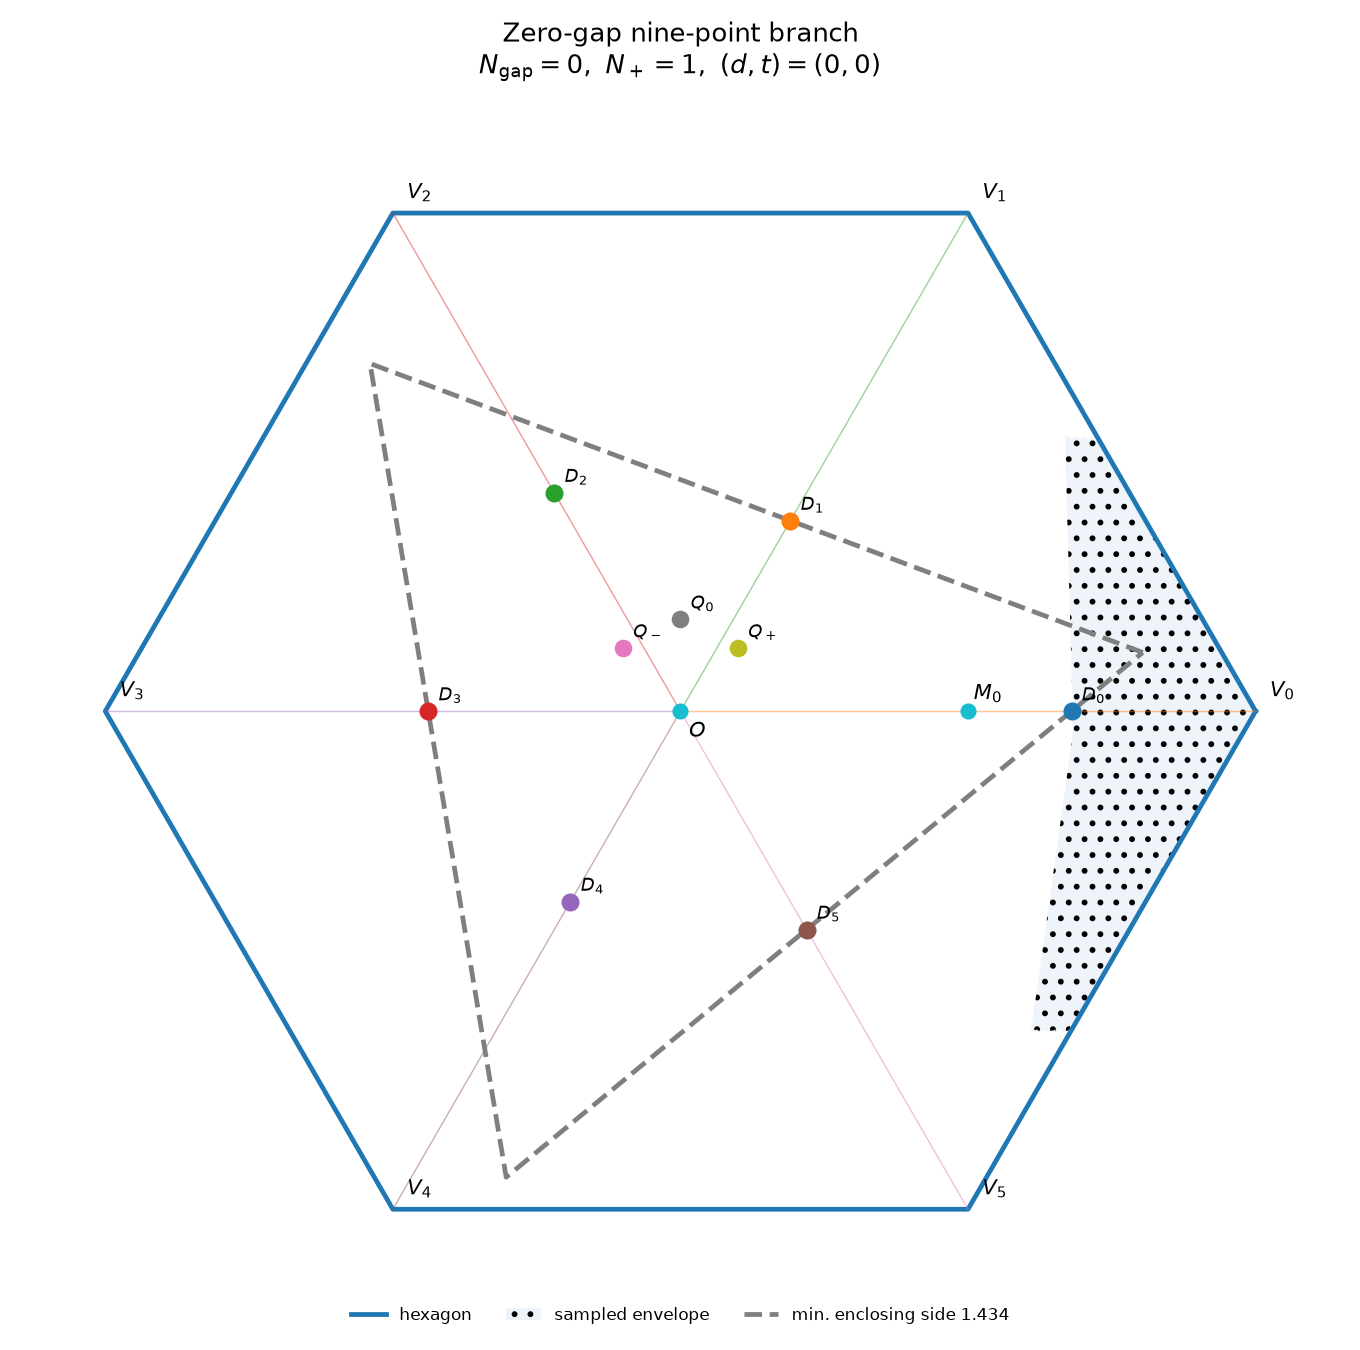
\includegraphics[width=\linewidth]{figures/trace_exact_ab/zero_gap_n1_vd0.png}
\textbf{(a)} Zero-gap nine-point branch.
\end{minipage}
\hfill
\begin{minipage}[t]{.485\linewidth}
\centering
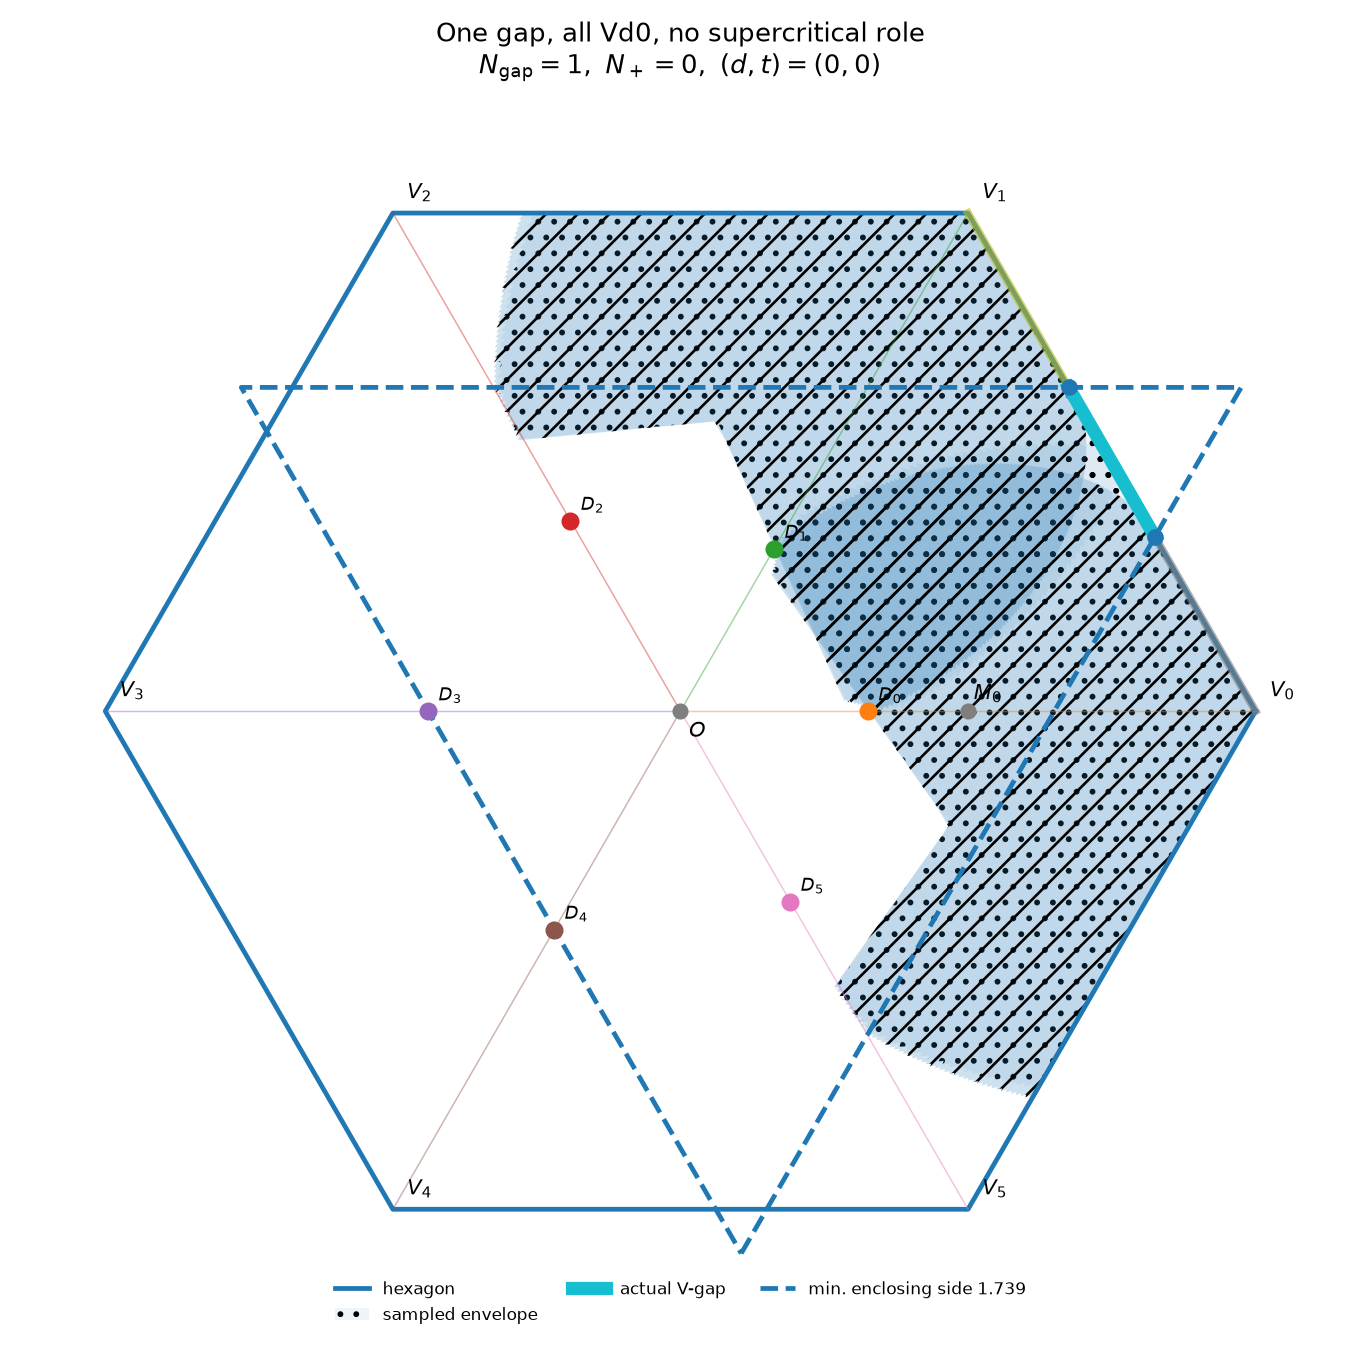
\includegraphics[width=\linewidth]{figures/trace_exact_ab/one_gap_n0_vd0.png}
\textbf{(b)} One gap, all Vd0, no supercritical role.
\end{minipage}
\caption{Trace-exact AB-envelope snapshots: Zero-gap nine-point branch; One gap, all Vd0, no supercritical role.}
\label{fig:trace-exact-ab-atlas-1}
\end{figure}

\begin{figure}[p]
\centering
\begin{minipage}[t]{.485\linewidth}
\centering
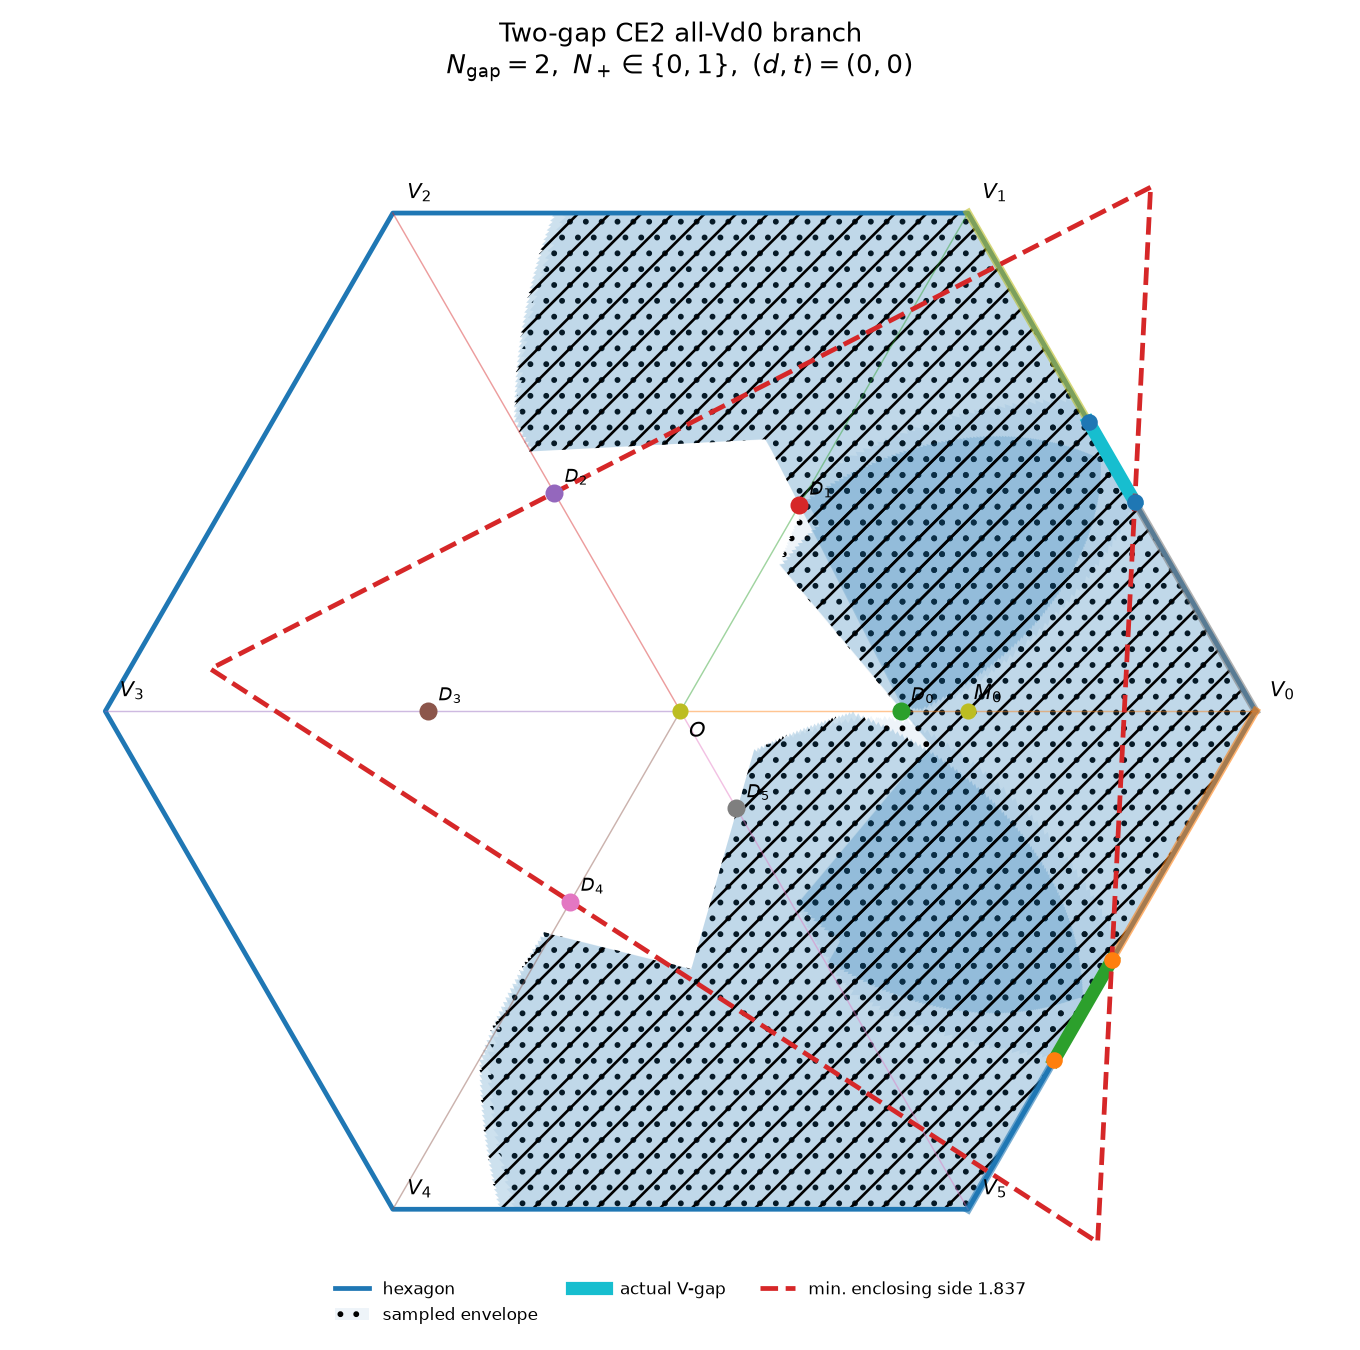
\includegraphics[width=\linewidth]{figures/trace_exact_ab/two_gap_vd0.png}
\textbf{(a)} Two-gap CE2 all-Vd0 branch.
\end{minipage}
\hfill
\begin{minipage}[t]{.485\linewidth}
\centering
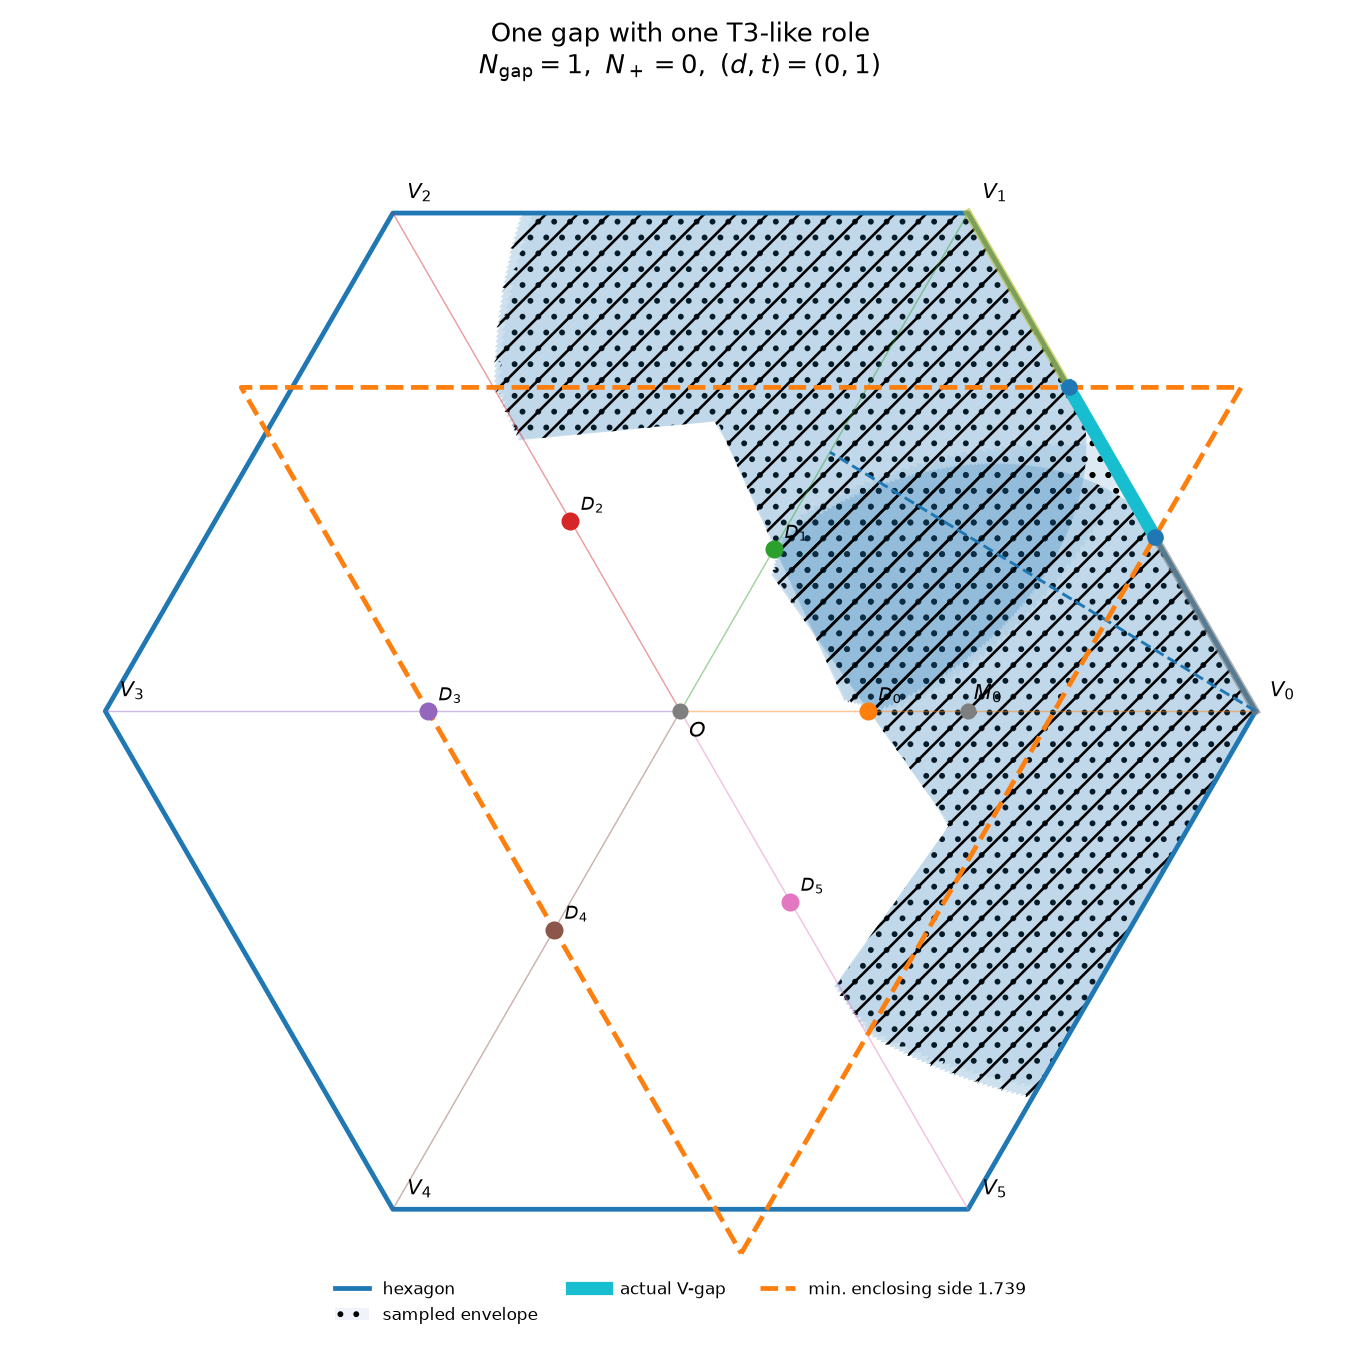
\includegraphics[width=\linewidth]{figures/trace_exact_ab/one_t3_n0.png}
\textbf{(b)} One gap with one T3-like role.
\end{minipage}
\caption{Trace-exact AB-envelope snapshots: Two-gap CE2 all-Vd0 branch; One gap with one T3-like role.}
\label{fig:trace-exact-ab-atlas-2}
\end{figure}

\begin{figure}[p]
\centering
\begin{minipage}[t]{.485\linewidth}
\centering
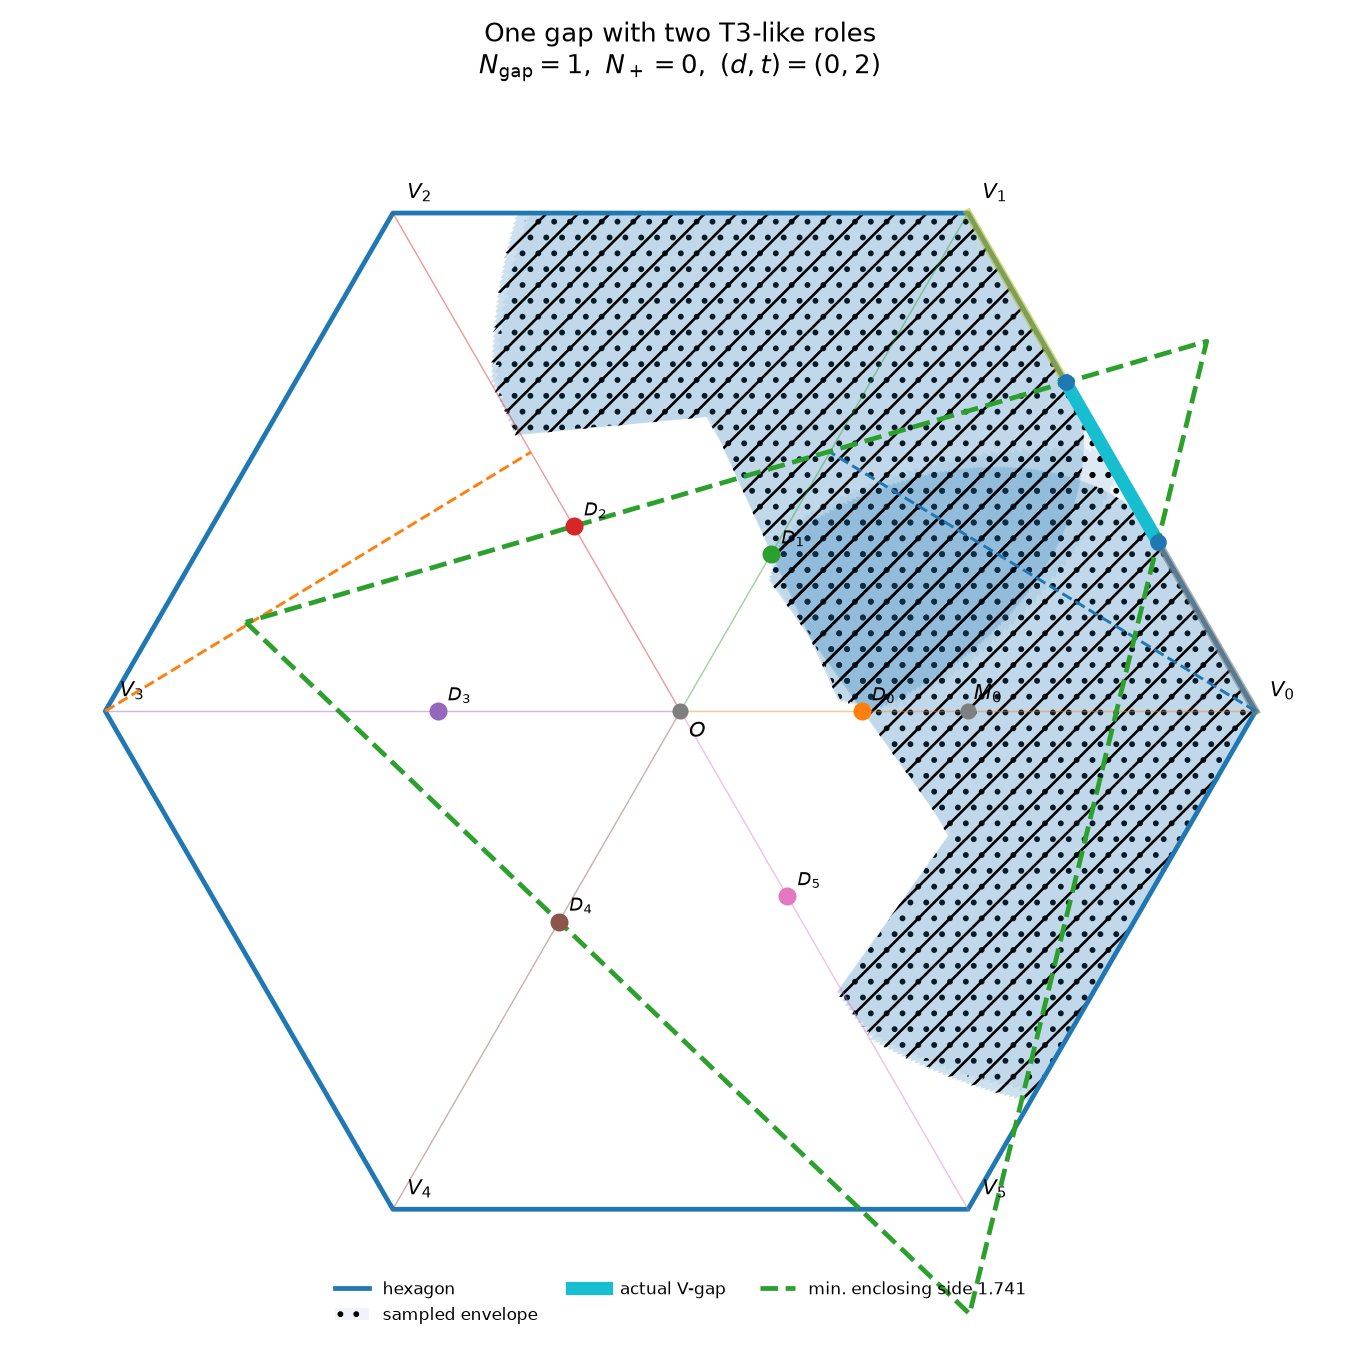
\includegraphics[width=\linewidth]{figures/trace_exact_ab/two_t3_n0.png}
\textbf{(a)} One gap with two T3-like roles.
\end{minipage}
\hfill
\begin{minipage}[t]{.485\linewidth}
\centering
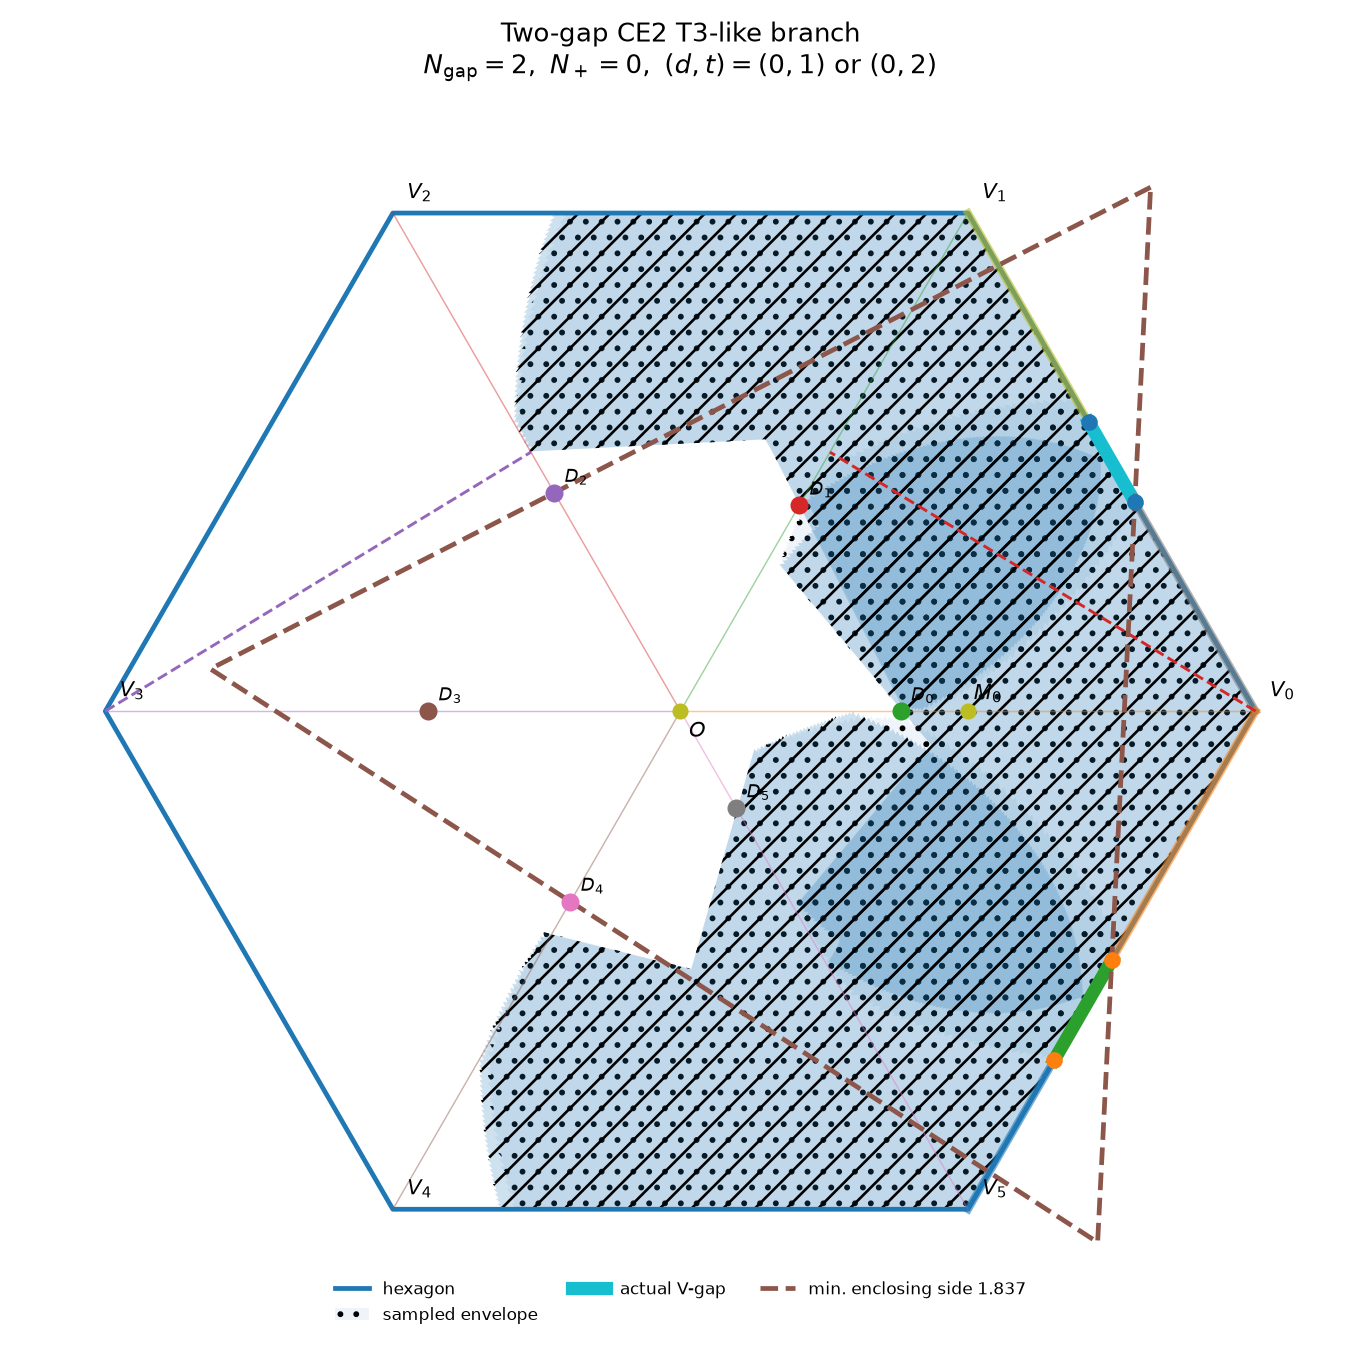
\includegraphics[width=\linewidth]{figures/trace_exact_ab/two_gap_t3_n0.png}
\textbf{(b)} Two-gap CE2 T3-like branch.
\end{minipage}
\caption{Trace-exact AB-envelope snapshots: One gap with two T3-like roles; Two-gap CE2 T3-like branch.}
\label{fig:trace-exact-ab-atlas-3}
\end{figure}

\begin{figure}[p]
\centering
\begin{minipage}[t]{.485\linewidth}
\centering
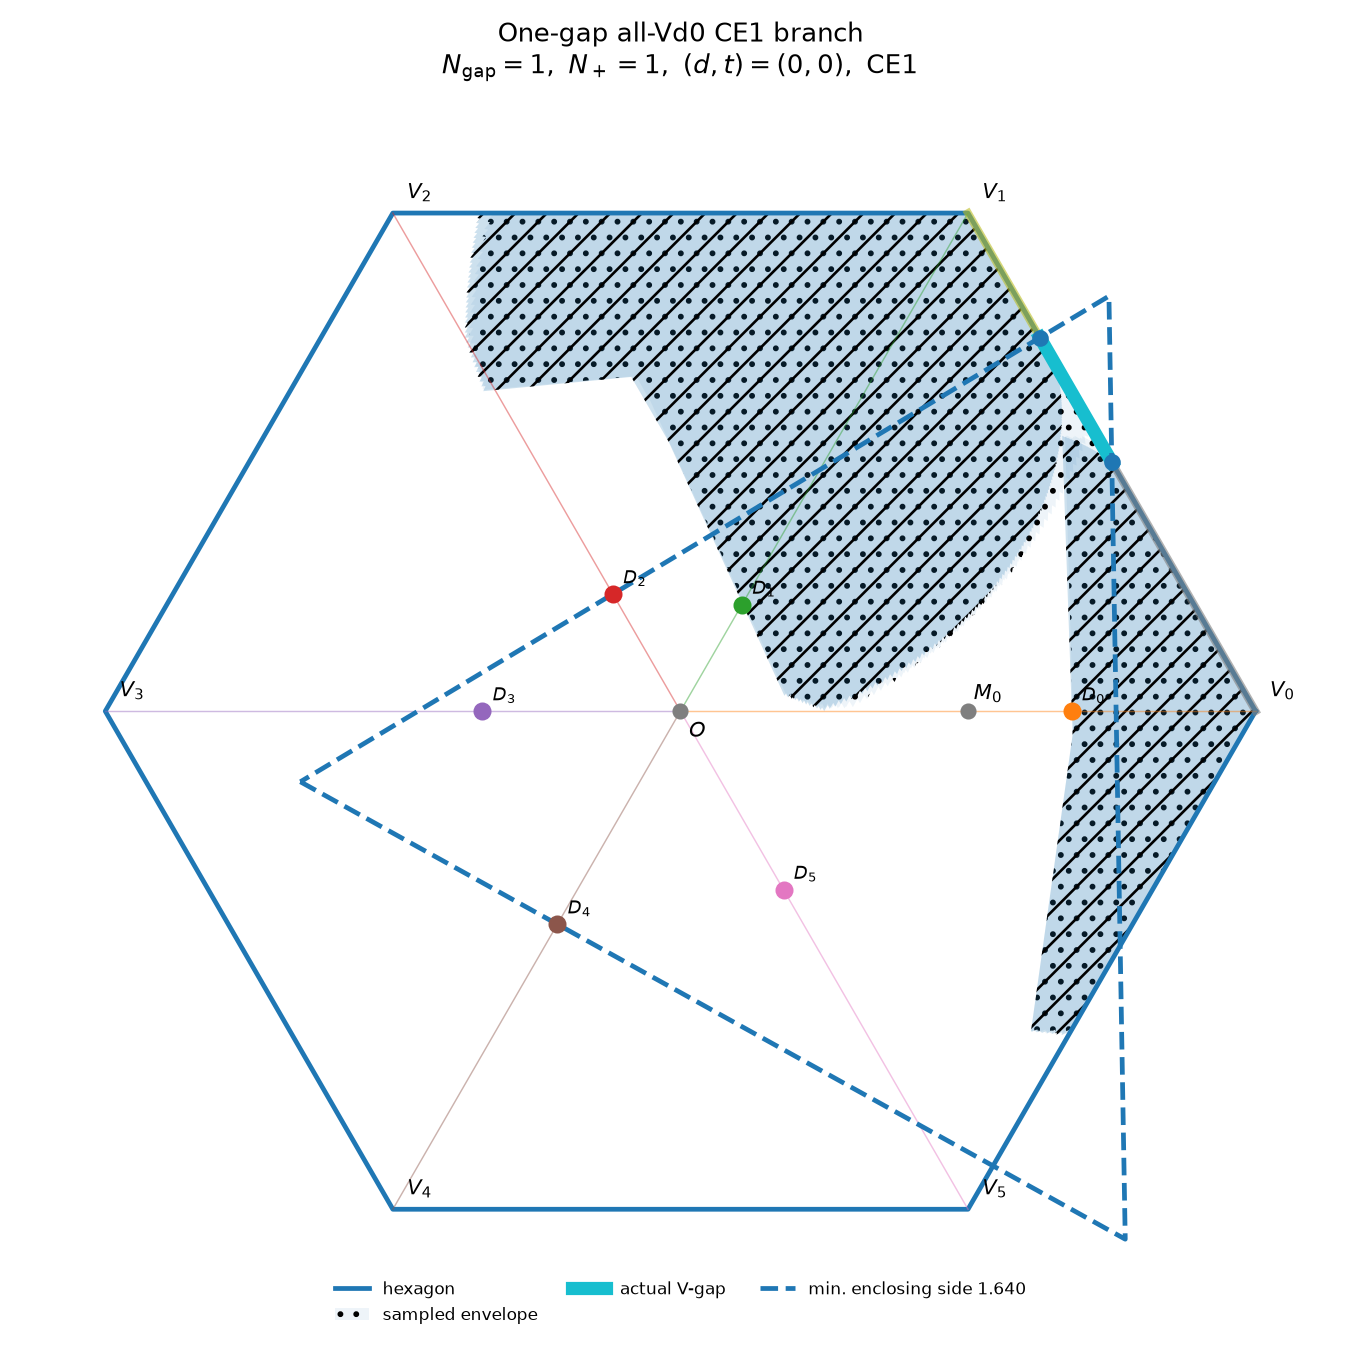
\includegraphics[width=\linewidth]{figures/trace_exact_ab/one_gap_n1_vd0_ce1.png}
\textbf{(a)} One-gap all-Vd0 CE1 branch.
\end{minipage}
\hfill
\begin{minipage}[t]{.485\linewidth}
\centering
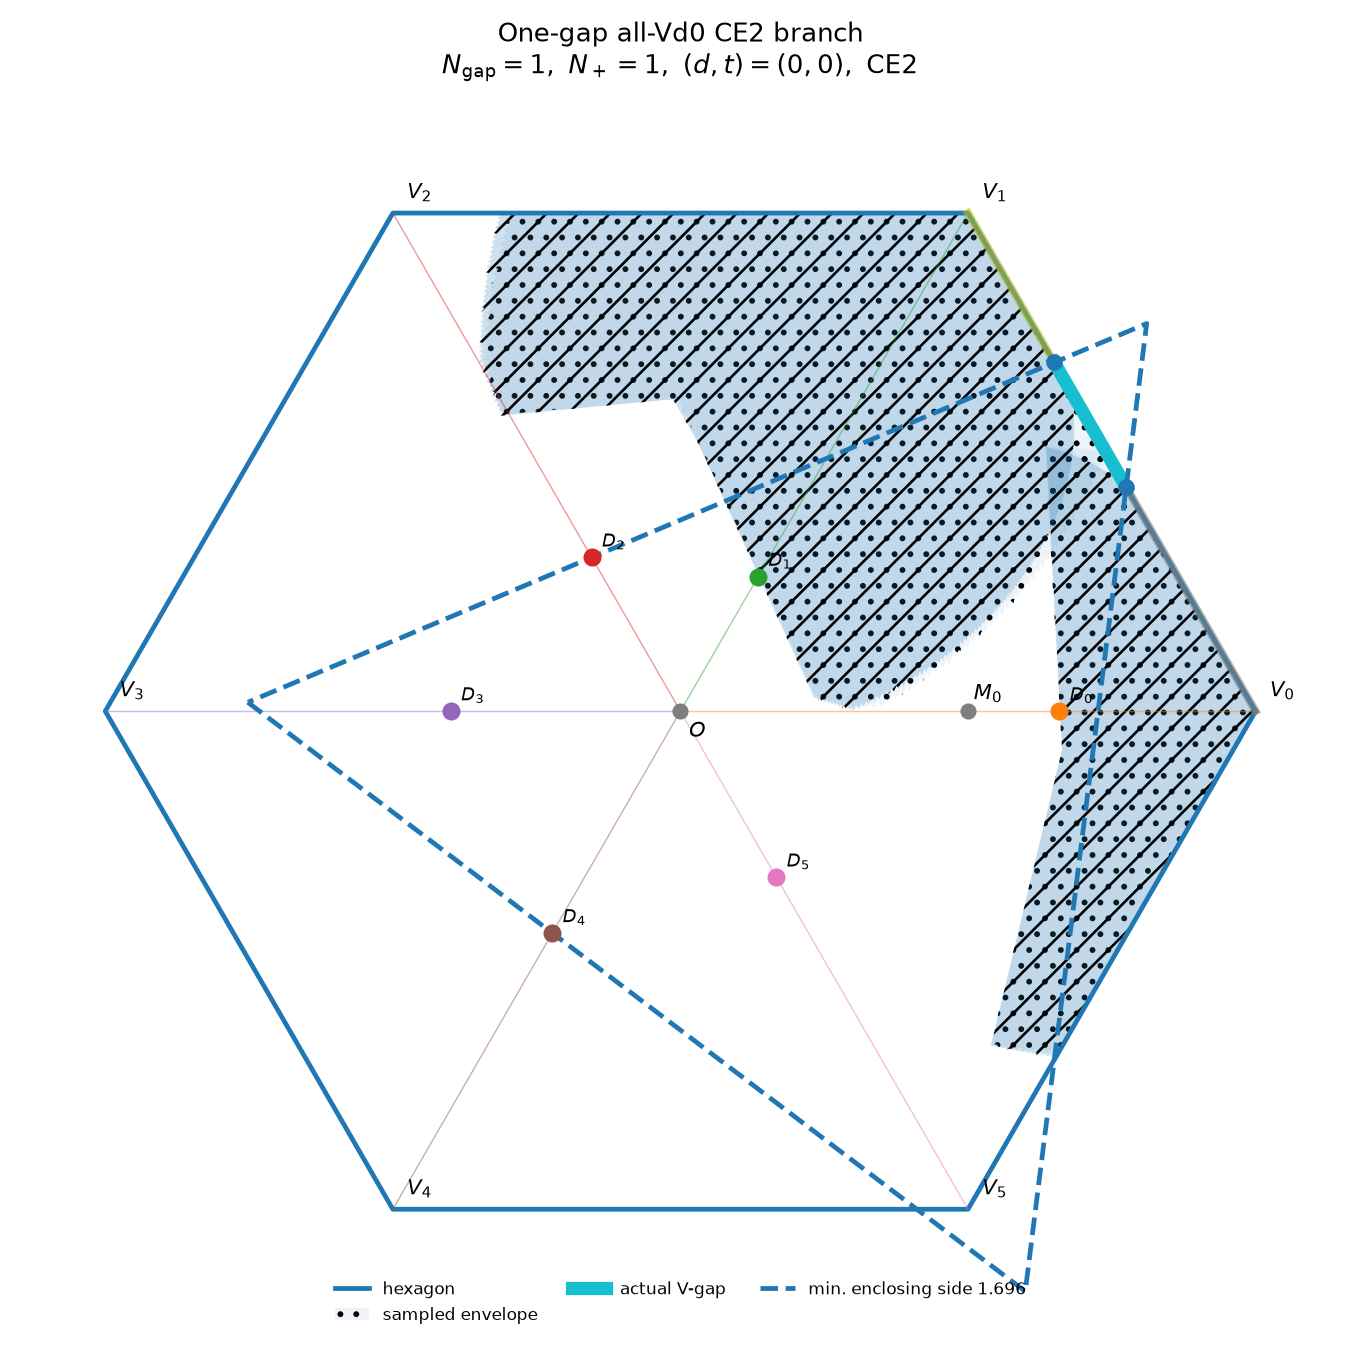
\includegraphics[width=\linewidth]{figures/trace_exact_ab/one_gap_n1_vd0_ce2.png}
\textbf{(b)} One-gap all-Vd0 CE2 branch.
\end{minipage}
\caption{Trace-exact AB-envelope snapshots: One-gap all-Vd0 CE1 branch; One-gap all-Vd0 CE2 branch.}
\label{fig:trace-exact-ab-atlas-4}
\end{figure}

\begin{figure}[p]
\centering
\begin{minipage}[t]{.485\linewidth}
\centering
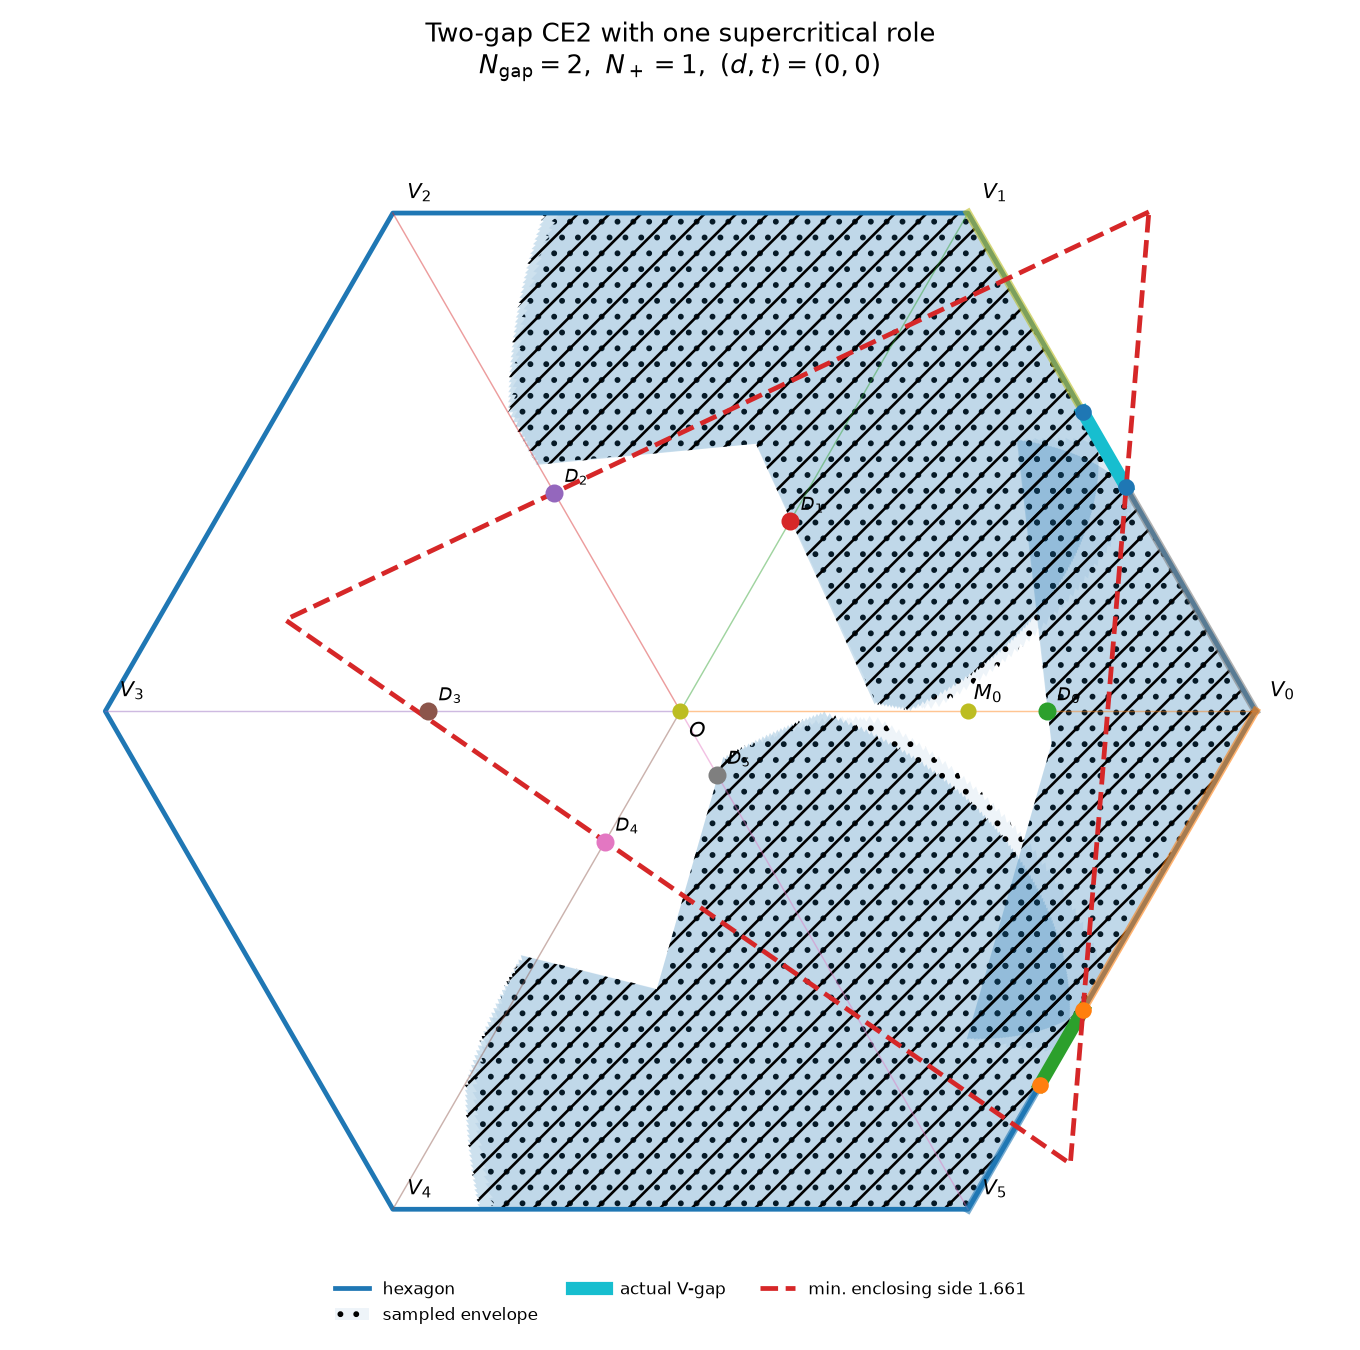
\includegraphics[width=\linewidth]{figures/trace_exact_ab/two_gap_n1_vd0.png}
\textbf{(a)} Two-gap CE2 with one supercritical role.
\end{minipage}
\hfill
\begin{minipage}[t]{.485\linewidth}
\centering
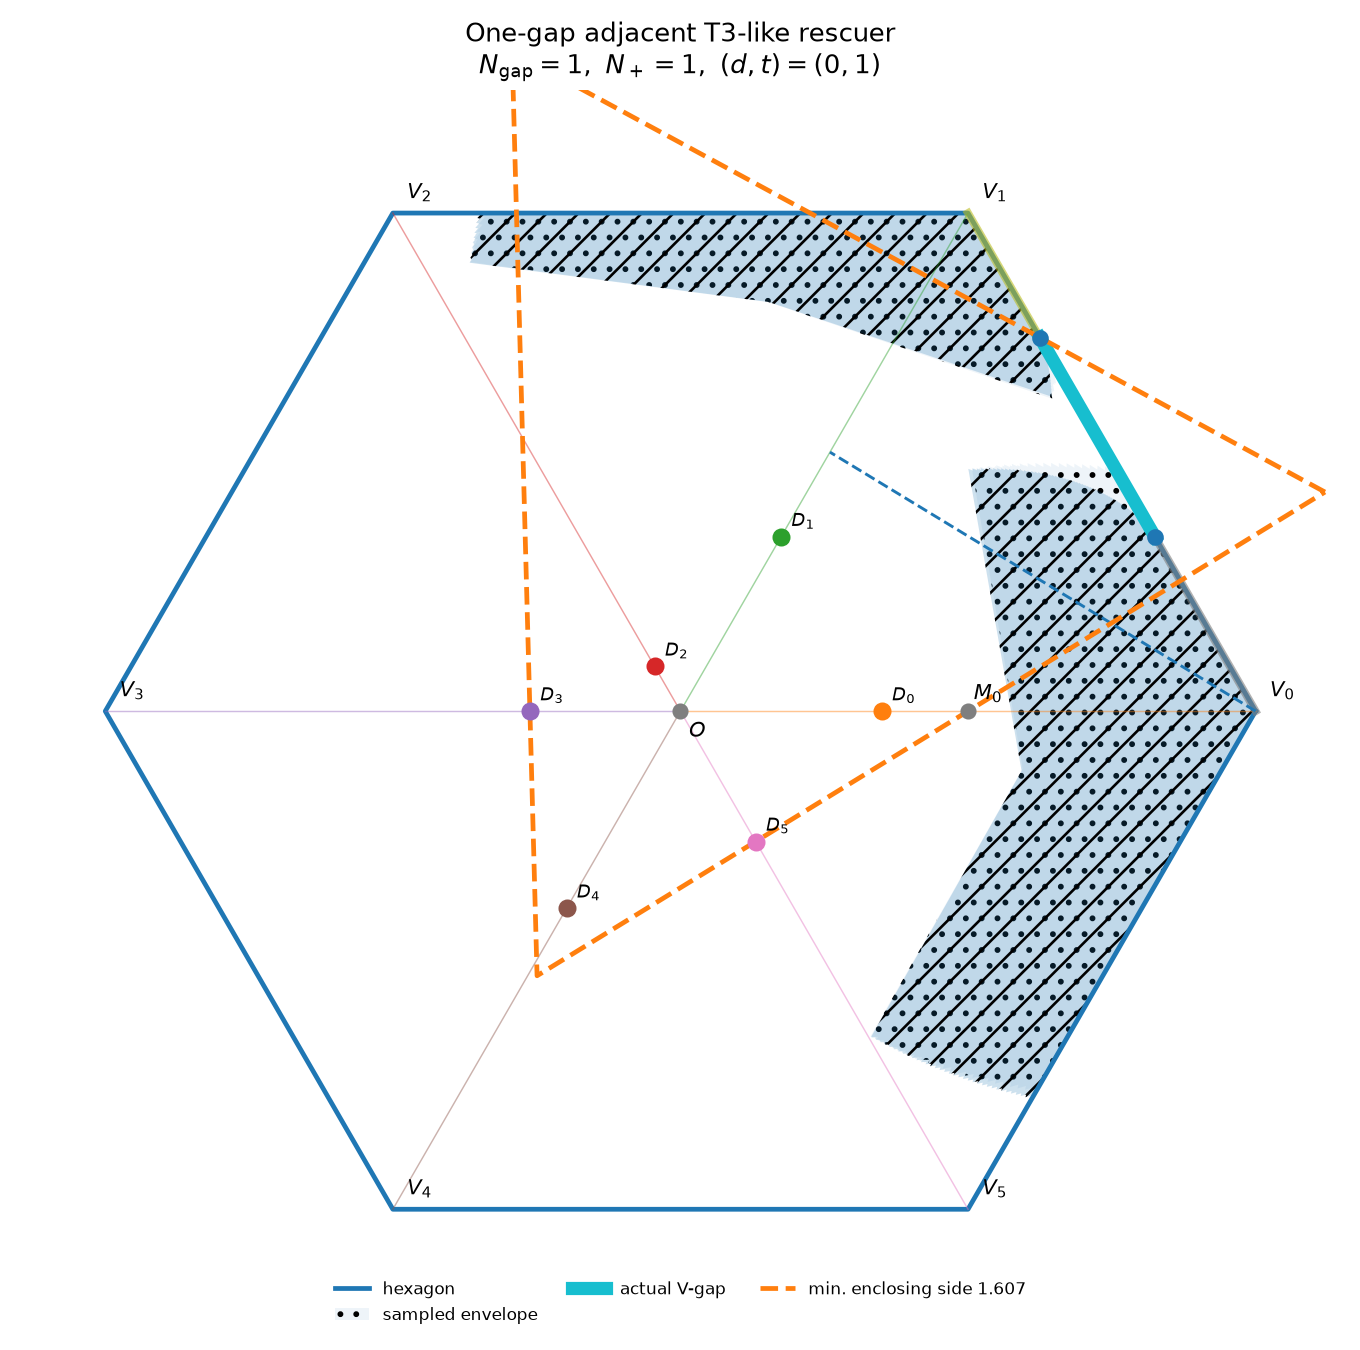
\includegraphics[width=\linewidth]{figures/trace_exact_ab/one_gap_n1_t3.png}
\textbf{(b)} One-gap adjacent T3-like rescuer.
\end{minipage}
\caption{Trace-exact AB-envelope snapshots: Two-gap CE2 with one supercritical role; One-gap adjacent T3-like rescuer.}
\label{fig:trace-exact-ab-atlas-5}
\end{figure}

\begin{figure}[p]
\centering
\begin{minipage}[t]{.485\linewidth}
\centering
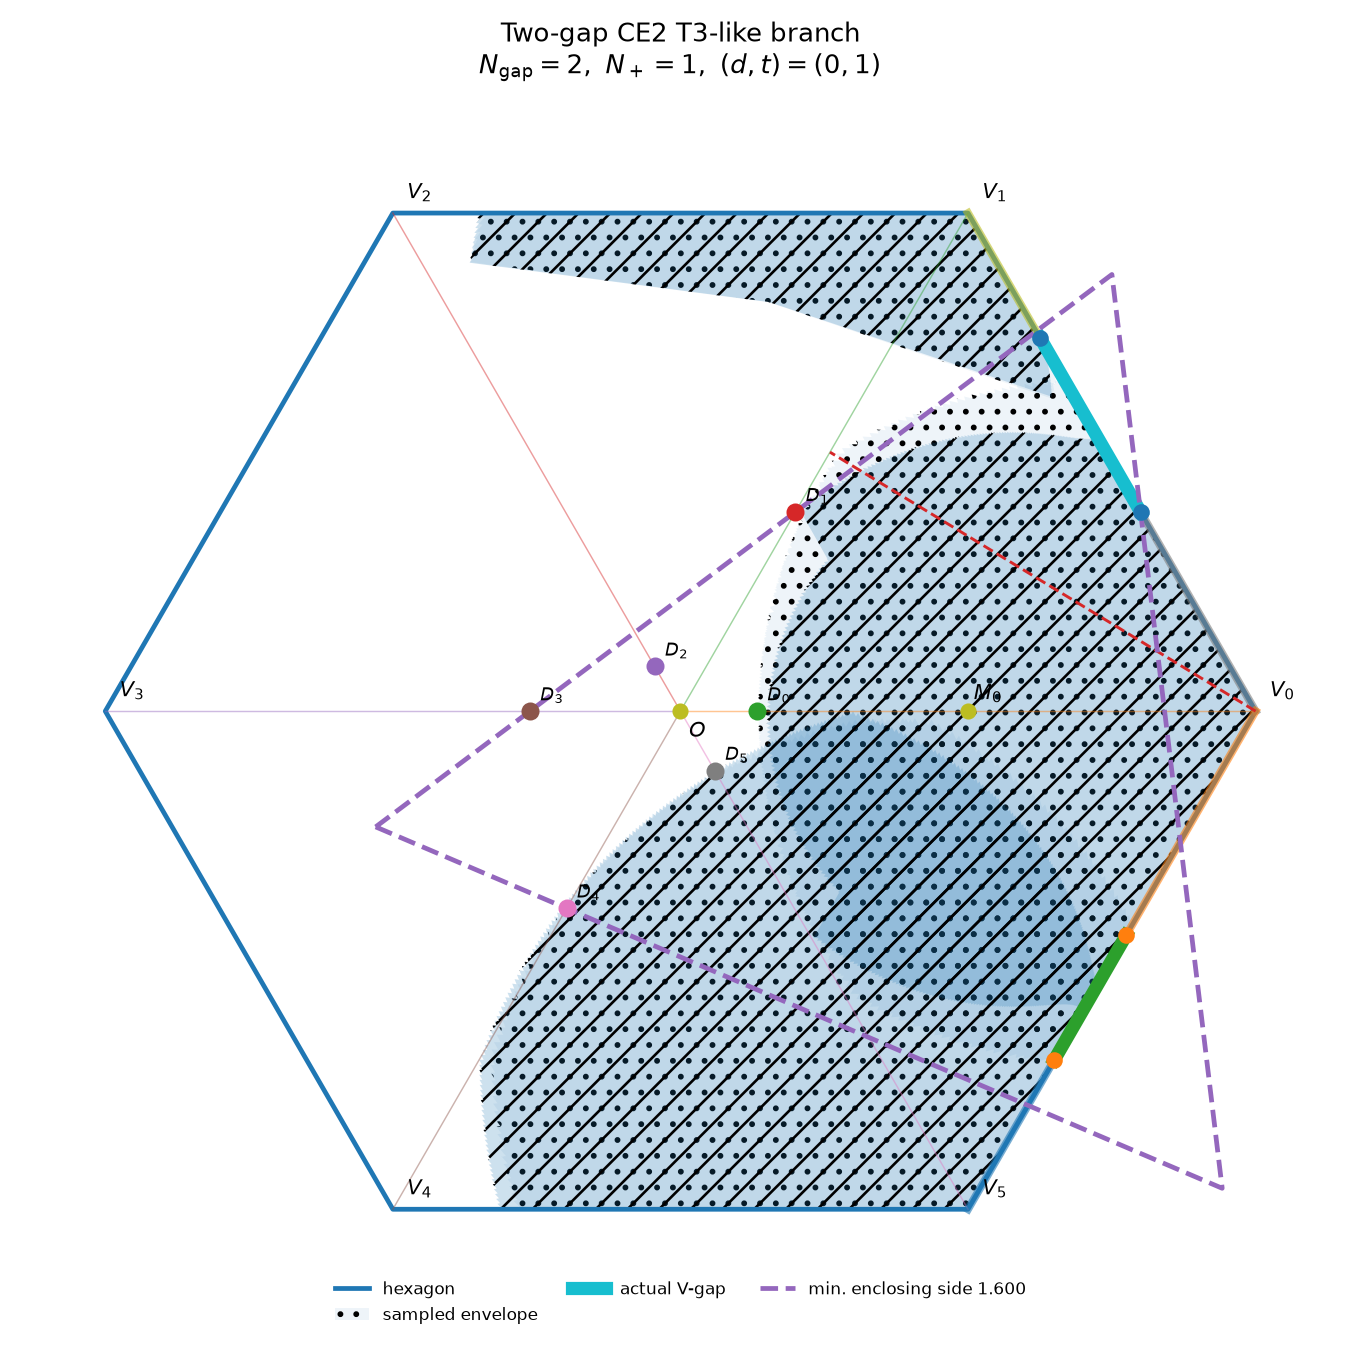
\includegraphics[width=\linewidth]{figures/trace_exact_ab/two_gap_n1_t3.png}
\textbf{(a)} Two-gap CE2 T3-like branch.
\end{minipage}
\hfill
\begin{minipage}[t]{.485\linewidth}
\centering
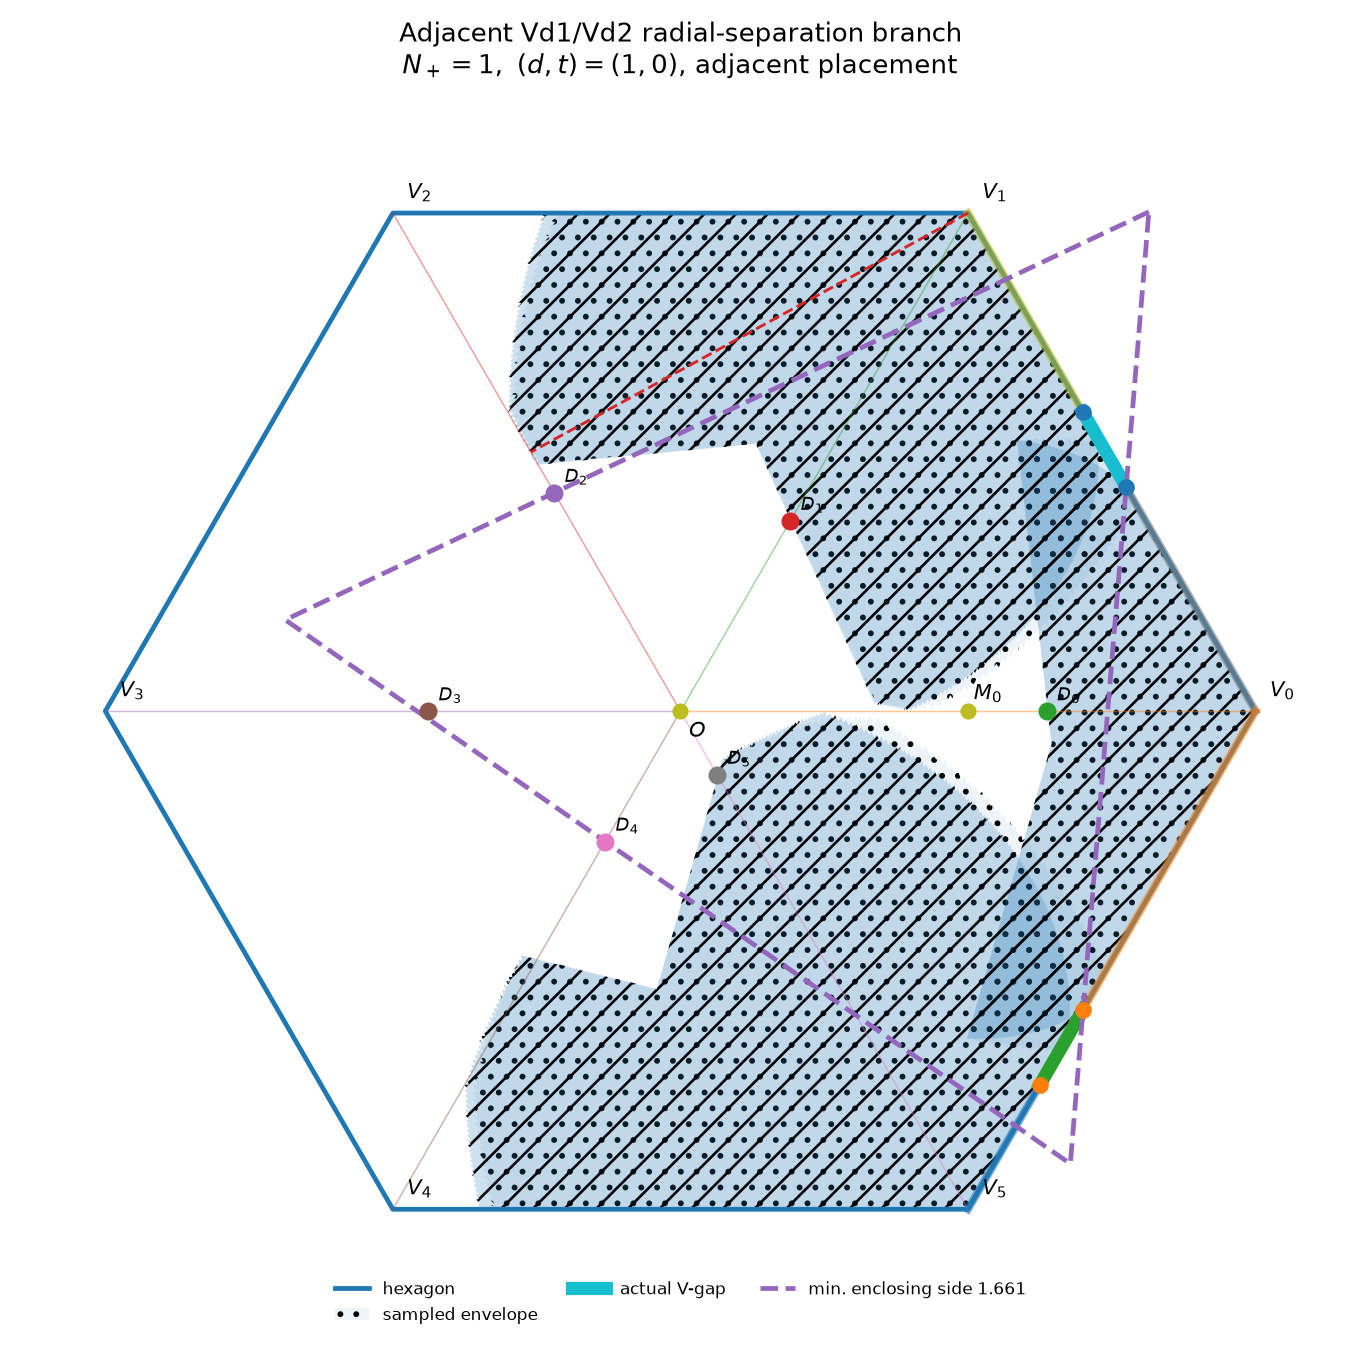
\includegraphics[width=\linewidth]{figures/trace_exact_ab/adjacent_vd.png}
\textbf{(b)} Adjacent Vd1/Vd2 radial-separation branch.
\end{minipage}
\caption{Trace-exact AB-envelope snapshots: Two-gap CE2 T3-like branch; Adjacent Vd1/Vd2 radial-separation branch.}
\label{fig:trace-exact-ab-atlas-6}
\end{figure}

\begin{figure}[p]
\centering
\begin{minipage}[t]{.485\linewidth}
\centering
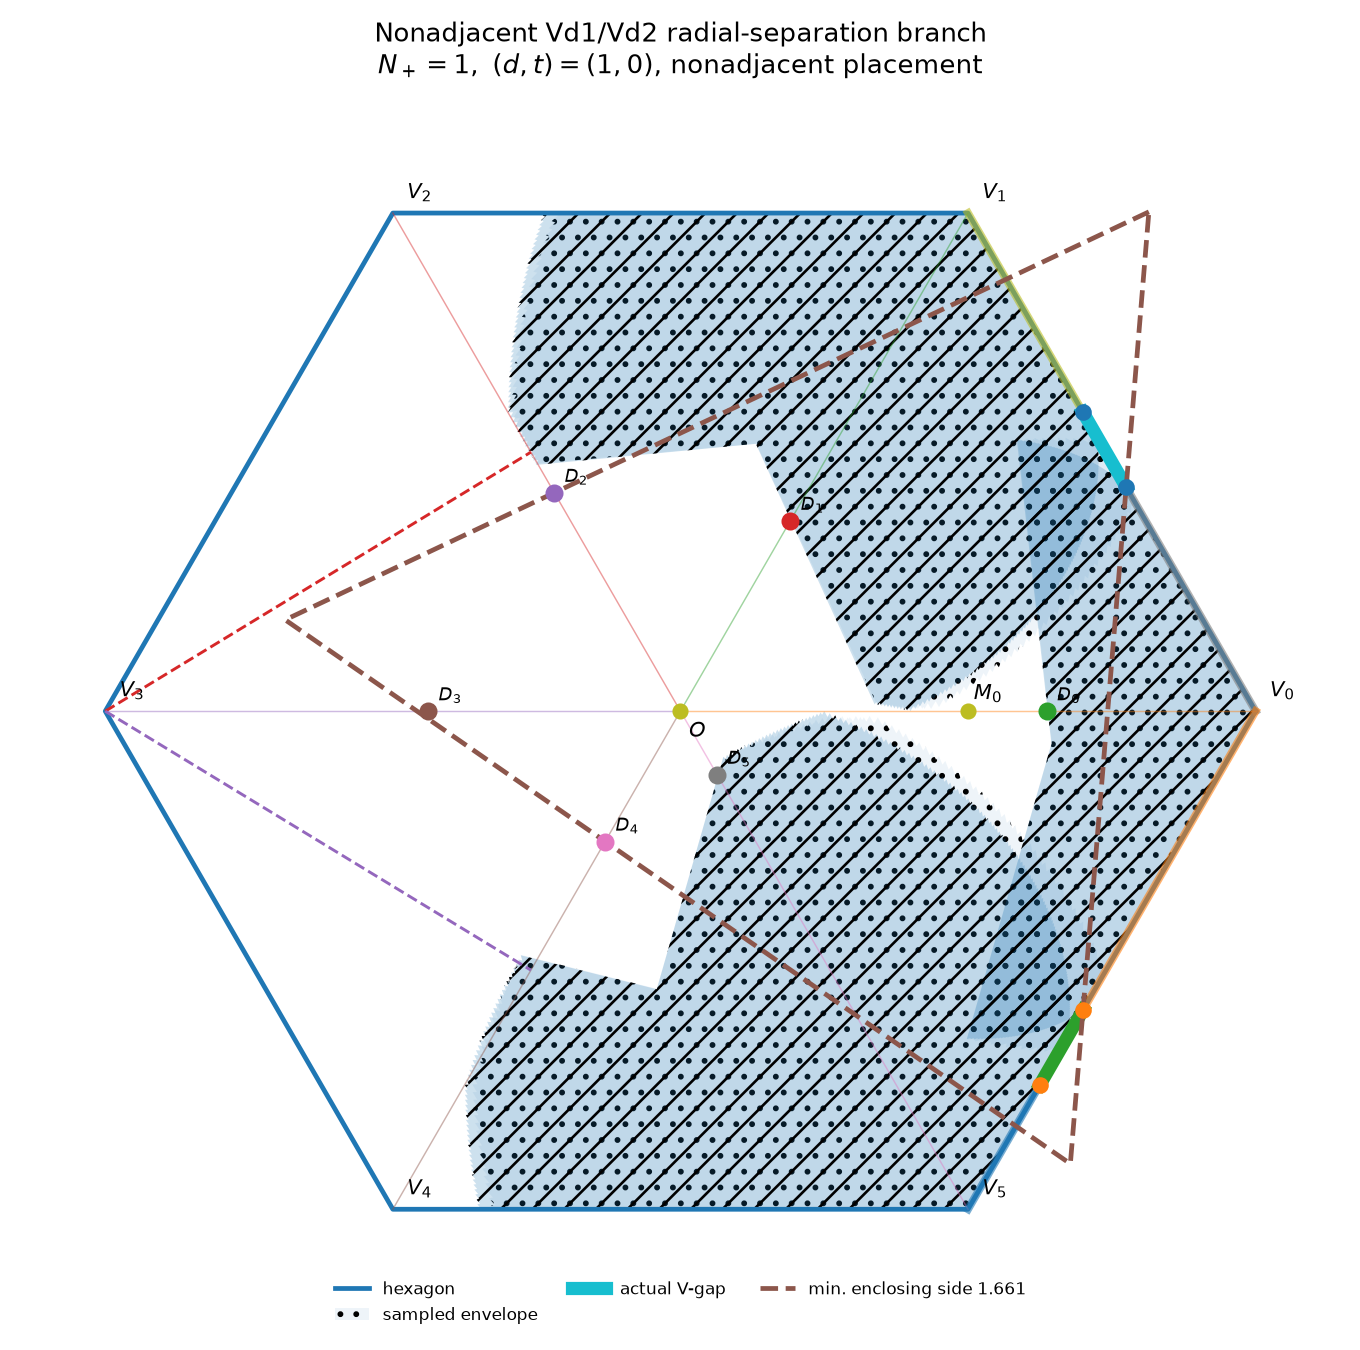
\includegraphics[width=\linewidth]{figures/trace_exact_ab/nonadjacent_vd.png}
\textbf{(a)} Nonadjacent Vd1/Vd2 radial-separation branch.
\end{minipage}
\hfill
\begin{minipage}[t]{.485\linewidth}
\centering
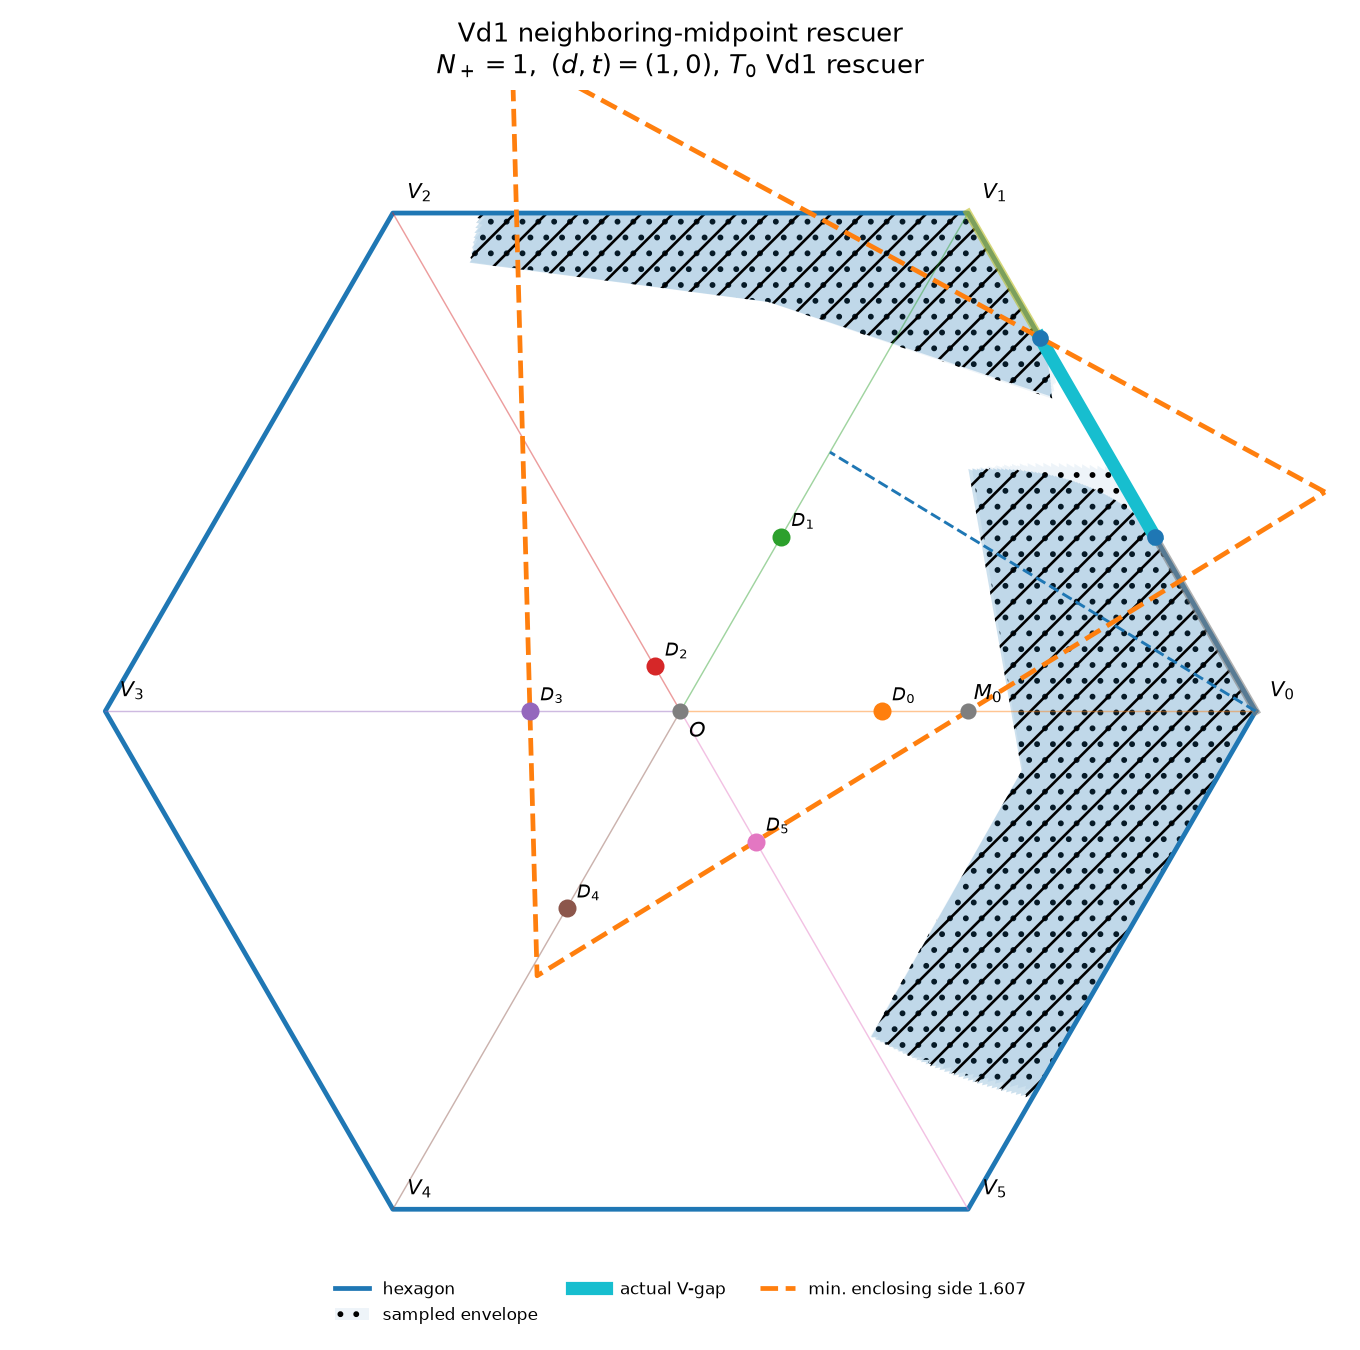
\includegraphics[width=\linewidth]{figures/trace_exact_ab/vd1_rescuer.png}
\textbf{(b)} Vd1 neighboring-midpoint rescuer.
\end{minipage}
\caption{Trace-exact AB-envelope snapshots: Nonadjacent Vd1/Vd2 radial-separation branch; Vd1 neighboring-midpoint rescuer.}
\label{fig:trace-exact-ab-atlas-7}
\end{figure}

\begin{figure}[p]
\centering
\begin{minipage}[t]{.485\linewidth}
\centering
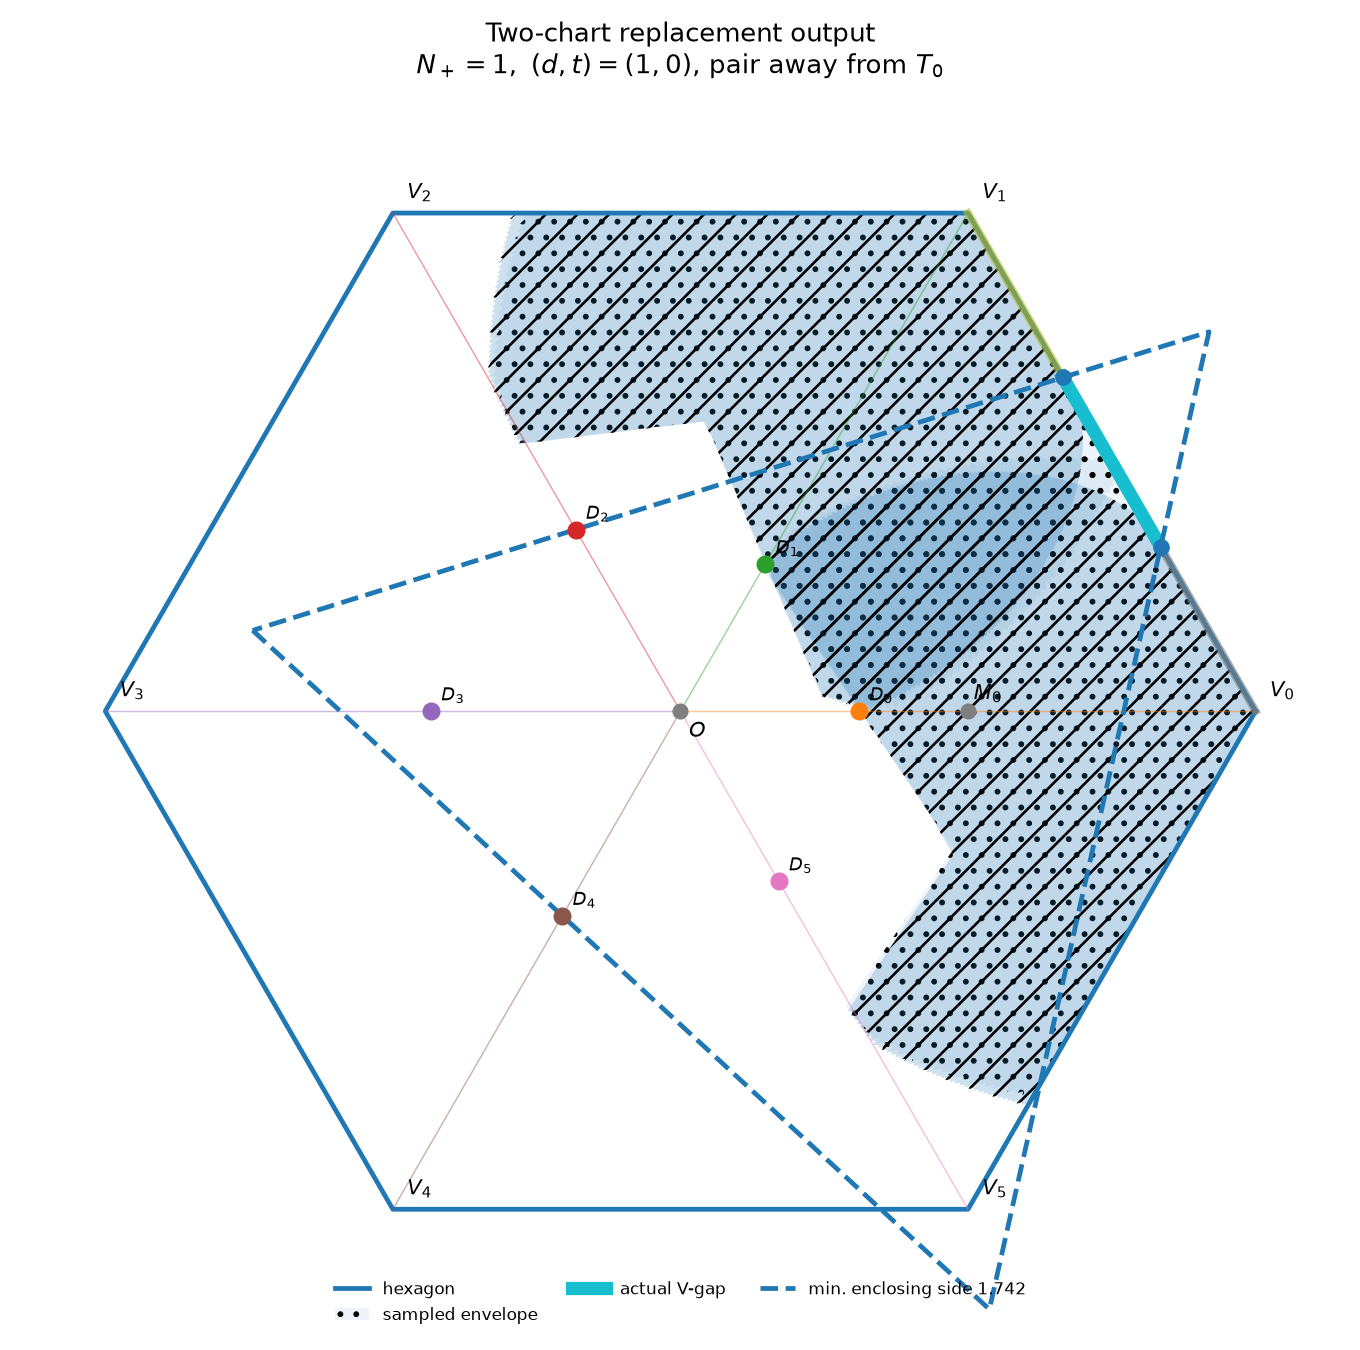
\includegraphics[width=\linewidth]{figures/trace_exact_ab/replacement_output.png}
\textbf{(a)} Two-chart replacement output.
\end{minipage}
\caption{Trace-exact AB-envelope snapshots: Two-chart replacement output.}
\label{fig:trace-exact-ab-atlas-8}
\end{figure}

